\begin{frame}
\frametitle{Inserting 1}
\begin{center}

	\tikzset{every picture/.style={line width=0.75pt}} %set default line width to 0.75pt

	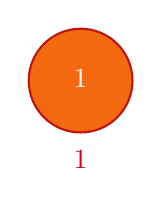
\begin{tikzpicture}[x=0.75pt,y=0.75pt,yscale=-1,xscale=1]
	%uncomment if require: \path (0,300); %set diagram left start at 0, and has height of 300

	\draw  [color={rgb, 255:red, 189; green, 19; blue, 19 }  ,draw opacity=1 ][fill={rgb, 255:red, 244; green, 105; blue, 16 }  ,fill opacity=1 ]  (321, 32) circle [x radius= 25, y radius= 25]  ;

	\draw (321,31) node [color={rgb, 255:red, 255; green, 255; blue, 255 }  ,opacity=1 ] [align=left] {1};
	\draw (321,70) node [color={rgb, 255:red, 208; green, 2; blue, 27 }  ,opacity=1 ] [align=left] {1};

	\end{tikzpicture}

\end{center}
\end{frame}



\begin{frame}
	\frametitle{Inserting 8}
	\begin{center}
			\tikzset{every picture/.style={line width=0.75pt}} %set default line width to 0.75pt

		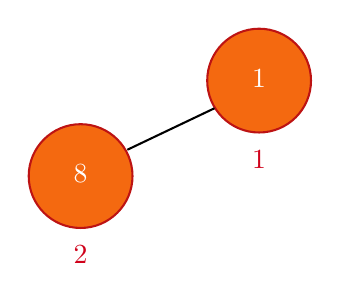
\begin{tikzpicture}[x=0.75pt,y=0.75pt,yscale=-1,xscale=1]
		%uncomment if require: \path (0,300); %set diagram left start at 0, and has height of 300

		\draw  [color={rgb, 255:red, 189; green, 19; blue, 19 }  ,draw opacity=1 ][fill={rgb, 255:red, 244; green, 105; blue, 16 }  ,fill opacity=1 ]  (321, 32) circle [x radius= 25, y radius= 25]  ;
		\draw  [color={rgb, 255:red, 189; green, 19; blue, 19 }  ,draw opacity=1 ][fill={rgb, 255:red, 244; green, 105; blue, 16 }  ,fill opacity=1 ]  (235, 78) circle [x radius= 25, y radius= 25]  ;
		\draw    (257.5,65.33) -- (299.5,45.33) ;



		\draw (321,31) node [color={rgb, 255:red, 255; green, 255; blue, 255 }  ,opacity=1 ] [align=left] {1};
		\draw (321,70) node [color={rgb, 255:red, 208; green, 2; blue, 27 }  ,opacity=1 ] [align=left] {1};
		\draw (235,77) node [color={rgb, 255:red, 255; green, 255; blue, 255 }  ,opacity=1 ] [align=left] {8};
		\draw (235,116) node [color={rgb, 255:red, 208; green, 2; blue, 27 }  ,opacity=1 ] [align=left] {2};


		\end{tikzpicture}
	\end{center}
\end{frame}



\begin{frame}
		\frametitle{Heapify()}
	\begin{center}
		\tikzset{every picture/.style={line width=0.75pt}} %set default line width to 0.75pt

		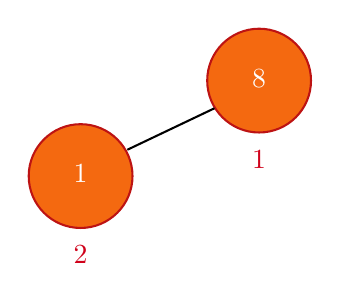
\begin{tikzpicture}[x=0.75pt,y=0.75pt,yscale=-1,xscale=1]
		%uncomment if require: \path (0,300); %set diagram left start at 0, and has height of 300

		\draw  [color={rgb, 255:red, 189; green, 19; blue, 19 }  ,draw opacity=1 ][fill={rgb, 255:red, 244; green, 105; blue, 16 }  ,fill opacity=1 ]  (321, 32) circle [x radius= 25, y radius= 25]  ;
		\draw  [color={rgb, 255:red, 189; green, 19; blue, 19 }  ,draw opacity=1 ][fill={rgb, 255:red, 244; green, 105; blue, 16 }  ,fill opacity=1 ]  (235, 78) circle [x radius= 25, y radius= 25]  ;
		\draw    (257.5,65.33) -- (299.5,45.33) ;



		\draw (321,31) node [color={rgb, 255:red, 255; green, 255; blue, 255 }  ,opacity=1 ] [align=left] {8};
		\draw (321,70) node [color={rgb, 255:red, 208; green, 2; blue, 27 }  ,opacity=1 ] [align=left] {1};
		\draw (235,77) node [color={rgb, 255:red, 255; green, 255; blue, 255 }  ,opacity=1 ] [align=left] {1};
		\draw (235,116) node [color={rgb, 255:red, 208; green, 2; blue, 27 }  ,opacity=1 ] [align=left] {2};


		\end{tikzpicture}

	\end{center}
\end{frame}


\begin{frame}
		\frametitle{Inserting 5}
	\begin{center}
		\tikzset{every picture/.style={line width=0.75pt}} %set default line width to 0.75pt

		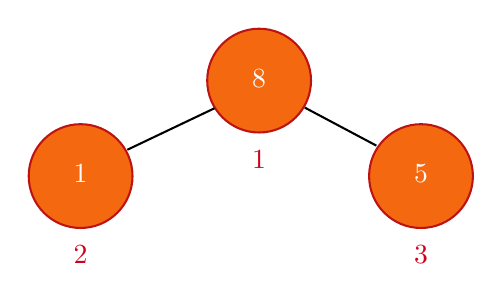
\begin{tikzpicture}[x=0.75pt,y=0.75pt,yscale=-1,xscale=1]
		%uncomment if require: \path (0,300); %set diagram left start at 0, and has height of 300

		\draw  [color={rgb, 255:red, 189; green, 19; blue, 19 }  ,draw opacity=1 ][fill={rgb, 255:red, 244; green, 105; blue, 16 }  ,fill opacity=1 ]  (321, 32) circle [x radius= 25, y radius= 25]  ;
		\draw  [color={rgb, 255:red, 189; green, 19; blue, 19 }  ,draw opacity=1 ][fill={rgb, 255:red, 244; green, 105; blue, 16 }  ,fill opacity=1 ]  (235, 78) circle [x radius= 25, y radius= 25]  ;
		\draw    (257.5,65.33) -- (299.5,45.33) ;


		\draw  [color={rgb, 255:red, 189; green, 19; blue, 19 }  ,draw opacity=1 ][fill={rgb, 255:red, 244; green, 105; blue, 16 }  ,fill opacity=1 ]  (399, 78) circle [x radius= 25, y radius= 25]  ;
		\draw    (343,45) -- (377.5,63.33) ;



		\draw (321,31) node [color={rgb, 255:red, 255; green, 255; blue, 255 }  ,opacity=1 ] [align=left] {8};
		\draw (321,70) node [color={rgb, 255:red, 208; green, 2; blue, 27 }  ,opacity=1 ] [align=left] {1};
		\draw (235,77) node [color={rgb, 255:red, 255; green, 255; blue, 255 }  ,opacity=1 ] [align=left] {1};
		\draw (235,116) node [color={rgb, 255:red, 208; green, 2; blue, 27 }  ,opacity=1 ] [align=left] {2};
		\draw (399,77) node [color={rgb, 255:red, 255; green, 255; blue, 255 }  ,opacity=1 ] [align=left] {5};
		\draw (399,116) node [color={rgb, 255:red, 208; green, 2; blue, 27 }  ,opacity=1 ] [align=left] {3};


		\end{tikzpicture}

	\end{center}
\end{frame}


\begin{frame}
	\frametitle{Inserting 2}
	\begin{center}
		\tikzset{every picture/.style={line width=0.75pt}} %set default line width to 0.75pt

		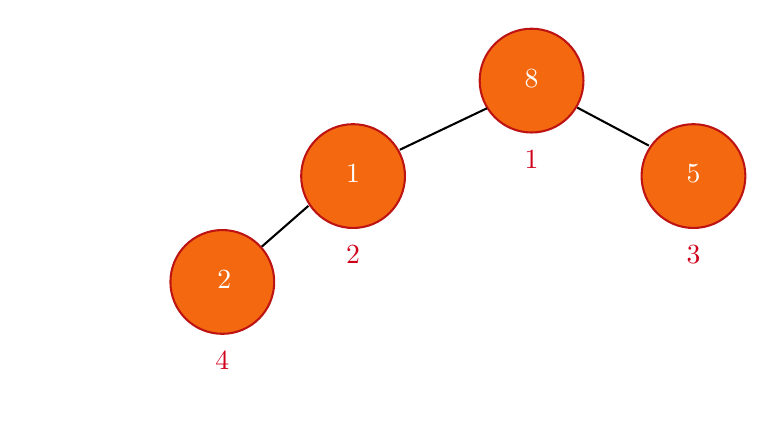
\begin{tikzpicture}[x=0.75pt,y=0.75pt,yscale=-1,xscale=1]
		%uncomment if require: \path (0,300); %set diagram left start at 0, and has height of 300

		\draw  [color={rgb, 255:red, 189; green, 19; blue, 19 }  ,draw opacity=1 ][fill={rgb, 255:red, 244; green, 105; blue, 16 }  ,fill opacity=1 ]  (321, 32) circle [x radius= 25, y radius= 25]  ;
		\draw  [color={rgb, 255:red, 189; green, 19; blue, 19 }  ,draw opacity=1 ][fill={rgb, 255:red, 244; green, 105; blue, 16 }  ,fill opacity=1 ]  (235, 78) circle [x radius= 25, y radius= 25]  ;
		\draw    (257.5,65.33) -- (299.5,45.33) ;


		\draw  [color={rgb, 255:red, 189; green, 19; blue, 19 }  ,draw opacity=1 ][fill={rgb, 255:red, 244; green, 105; blue, 16 }  ,fill opacity=1 ]  (399, 78) circle [x radius= 25, y radius= 25]  ;
		\draw    (343,45) -- (377.5,63.33) ;


		\draw  [color={rgb, 255:red, 189; green, 19; blue, 19 }  ,draw opacity=1 ][fill={rgb, 255:red, 244; green, 105; blue, 16 }  ,fill opacity=1 ]  (172, 129) circle [x radius= 25, y radius= 25]  ;
		\draw    (191,112) -- (213.5,92.33) ;



		\draw (321,31) node [color={rgb, 255:red, 255; green, 255; blue, 255 }  ,opacity=1 ] [align=left] {8};
		\draw (321,70) node [color={rgb, 255:red, 208; green, 2; blue, 27 }  ,opacity=1 ] [align=left] {1};
		\draw (235,77) node [color={rgb, 255:red, 255; green, 255; blue, 255 }  ,opacity=1 ] [align=left] {1};
		\draw (235,116) node [color={rgb, 255:red, 208; green, 2; blue, 27 }  ,opacity=1 ] [align=left] {2};
		\draw (399,77) node [color={rgb, 255:red, 255; green, 255; blue, 255 }  ,opacity=1 ] [align=left] {5};
		\draw (399,116) node [color={rgb, 255:red, 208; green, 2; blue, 27 }  ,opacity=1 ] [align=left] {3};
		\draw (173,128) node [color={rgb, 255:red, 255; green, 255; blue, 255 }  ,opacity=1 ] [align=left] {2};
		\draw (172,167) node [color={rgb, 255:red, 208; green, 2; blue, 27 }  ,opacity=1 ] [align=left] {4};
		\draw (86,174) node [color={rgb, 255:red, 255; green, 255; blue, 255 }  ,opacity=1 ] [align=left] {1};
		\draw (250,174) node [color={rgb, 255:red, 255; green, 255; blue, 255 }  ,opacity=1 ] [align=left] {5};


		\end{tikzpicture}
	\end{center}
\end{frame}


\begin{frame}
	\frametitle{Heapify()}
	\begin{center}
			\tikzset{every picture/.style={line width=0.75pt}} %set default line width to 0.75pt

		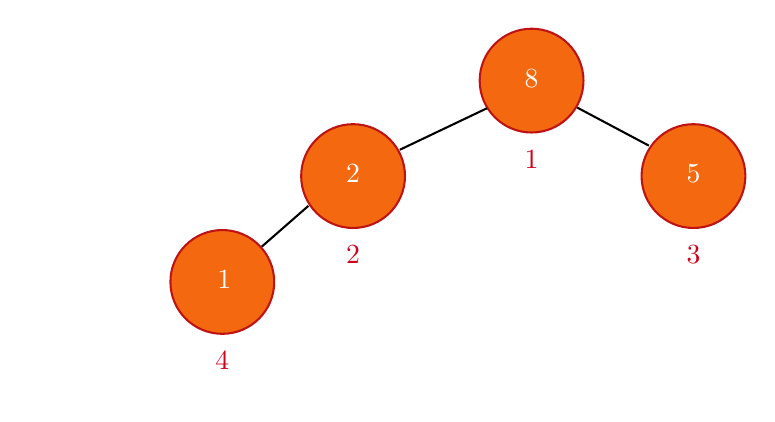
\begin{tikzpicture}[x=0.75pt,y=0.75pt,yscale=-1,xscale=1]
		%uncomment if require: \path (0,300); %set diagram left start at 0, and has height of 300

		\draw  [color={rgb, 255:red, 189; green, 19; blue, 19 }  ,draw opacity=1 ][fill={rgb, 255:red, 244; green, 105; blue, 16 }  ,fill opacity=1 ]  (321, 32) circle [x radius= 25, y radius= 25]  ;
		\draw  [color={rgb, 255:red, 189; green, 19; blue, 19 }  ,draw opacity=1 ][fill={rgb, 255:red, 244; green, 105; blue, 16 }  ,fill opacity=1 ]  (235, 78) circle [x radius= 25, y radius= 25]  ;
		\draw    (257.5,65.33) -- (299.5,45.33) ;


		\draw  [color={rgb, 255:red, 189; green, 19; blue, 19 }  ,draw opacity=1 ][fill={rgb, 255:red, 244; green, 105; blue, 16 }  ,fill opacity=1 ]  (399, 78) circle [x radius= 25, y radius= 25]  ;
		\draw    (343,45) -- (377.5,63.33) ;


		\draw  [color={rgb, 255:red, 189; green, 19; blue, 19 }  ,draw opacity=1 ][fill={rgb, 255:red, 244; green, 105; blue, 16 }  ,fill opacity=1 ]  (172, 129) circle [x radius= 25, y radius= 25]  ;
		\draw    (191,112) -- (213.5,92.33) ;



		\draw (321,31) node [color={rgb, 255:red, 255; green, 255; blue, 255 }  ,opacity=1 ] [align=left] {8};
		\draw (321,70) node [color={rgb, 255:red, 208; green, 2; blue, 27 }  ,opacity=1 ] [align=left] {1};
		\draw (235,77) node [color={rgb, 255:red, 255; green, 255; blue, 255 }  ,opacity=1 ] [align=left] {2};
		\draw (235,116) node [color={rgb, 255:red, 208; green, 2; blue, 27 }  ,opacity=1 ] [align=left] {2};
		\draw (399,77) node [color={rgb, 255:red, 255; green, 255; blue, 255 }  ,opacity=1 ] [align=left] {5};
		\draw (399,116) node [color={rgb, 255:red, 208; green, 2; blue, 27 }  ,opacity=1 ] [align=left] {3};
		\draw (173,128) node [color={rgb, 255:red, 255; green, 255; blue, 255 }  ,opacity=1 ] [align=left] {1};
		\draw (172,167) node [color={rgb, 255:red, 208; green, 2; blue, 27 }  ,opacity=1 ] [align=left] {4};
		\draw (86,174) node [color={rgb, 255:red, 255; green, 255; blue, 255 }  ,opacity=1 ] [align=left] {1};
		\draw (250,174) node [color={rgb, 255:red, 255; green, 255; blue, 255 }  ,opacity=1 ] [align=left] {5};


		\end{tikzpicture}
	\end{center}
\end{frame}

\begin{frame}
	\frametitle{Inserting 9}

   \begin{center}
   	\tikzset{every picture/.style={line width=0.75pt}} %set default line width to 0.75pt

   	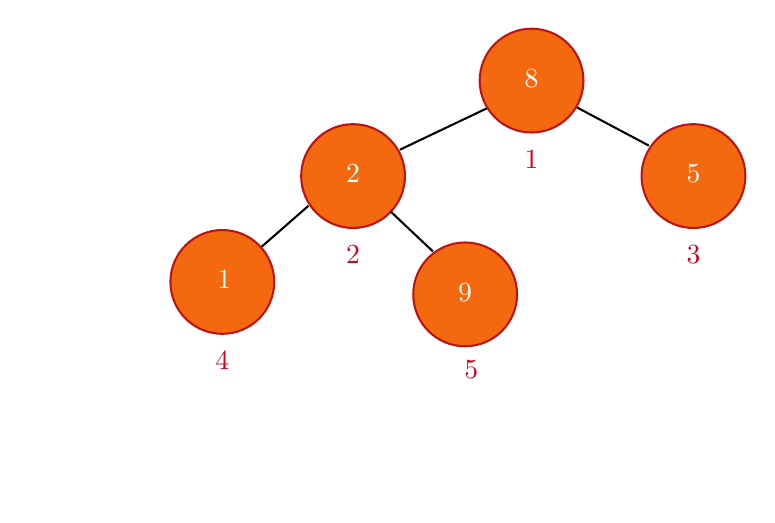
\begin{tikzpicture}[x=0.75pt,y=0.75pt,yscale=-1,xscale=1]
   	%uncomment if require: \path (0,300); %set diagram left start at 0, and has height of 300

   	\draw  [color={rgb, 255:red, 189; green, 19; blue, 19 }  ,draw opacity=1 ][fill={rgb, 255:red, 244; green, 105; blue, 16 }  ,fill opacity=1 ]  (321, 32) circle [x radius= 25, y radius= 25]  ;
   	\draw  [color={rgb, 255:red, 189; green, 19; blue, 19 }  ,draw opacity=1 ][fill={rgb, 255:red, 244; green, 105; blue, 16 }  ,fill opacity=1 ]  (235, 78) circle [x radius= 25, y radius= 25]  ;
   	\draw    (257.5,65.33) -- (299.5,45.33) ;


   	\draw  [color={rgb, 255:red, 189; green, 19; blue, 19 }  ,draw opacity=1 ][fill={rgb, 255:red, 244; green, 105; blue, 16 }  ,fill opacity=1 ]  (399, 78) circle [x radius= 25, y radius= 25]  ;
   	\draw    (343,45) -- (377.5,63.33) ;


   	\draw  [color={rgb, 255:red, 189; green, 19; blue, 19 }  ,draw opacity=1 ][fill={rgb, 255:red, 244; green, 105; blue, 16 }  ,fill opacity=1 ]  (172, 129) circle [x radius= 25, y radius= 25]  ;
   	\draw    (191,112) -- (213.5,92.33) ;


   	\draw  [color={rgb, 255:red, 189; green, 19; blue, 19 }  ,draw opacity=1 ][fill={rgb, 255:red, 244; green, 105; blue, 16 }  ,fill opacity=1 ]  (289, 135) circle [x radius= 25, y radius= 25]  ;
   	\draw    (253,95) -- (273.5,114.33) ;



   	\draw (321,31) node [color={rgb, 255:red, 255; green, 255; blue, 255 }  ,opacity=1 ] [align=left] {8};
   	\draw (321,70) node [color={rgb, 255:red, 208; green, 2; blue, 27 }  ,opacity=1 ] [align=left] {1};
   	\draw (235,77) node [color={rgb, 255:red, 255; green, 255; blue, 255 }  ,opacity=1 ] [align=left] {2};
   	\draw (235,116) node [color={rgb, 255:red, 208; green, 2; blue, 27 }  ,opacity=1 ] [align=left] {2};
   	\draw (399,77) node [color={rgb, 255:red, 255; green, 255; blue, 255 }  ,opacity=1 ] [align=left] {5};
   	\draw (399,116) node [color={rgb, 255:red, 208; green, 2; blue, 27 }  ,opacity=1 ] [align=left] {3};
   	\draw (173,128) node [color={rgb, 255:red, 255; green, 255; blue, 255 }  ,opacity=1 ] [align=left] {1};
   	\draw (172,167) node [color={rgb, 255:red, 208; green, 2; blue, 27 }  ,opacity=1 ] [align=left] {4};
   	\draw (86,174) node [color={rgb, 255:red, 255; green, 255; blue, 255 }  ,opacity=1 ] [align=left] {1};
   	\draw (250,174) node [color={rgb, 255:red, 255; green, 255; blue, 255 }  ,opacity=1 ] [align=left] {5};
   	\draw (289,134) node [color={rgb, 255:red, 255; green, 255; blue, 255 }  ,opacity=1 ] [align=left] {9};
   	\draw (292,171) node [color={rgb, 255:red, 208; green, 2; blue, 27 }  ,opacity=1 ] [align=left] {5};
   	\draw (304,223) node [color={rgb, 255:red, 255; green, 255; blue, 255 }  ,opacity=1 ] [align=left] {5};


   	\end{tikzpicture}
   \end{center}
\end{frame}


\begin{frame}
	\frametitle{Heapify()}

	\begin{center}
		\tikzset{every picture/.style={line width=0.75pt}} %set default line width to 0.75pt

		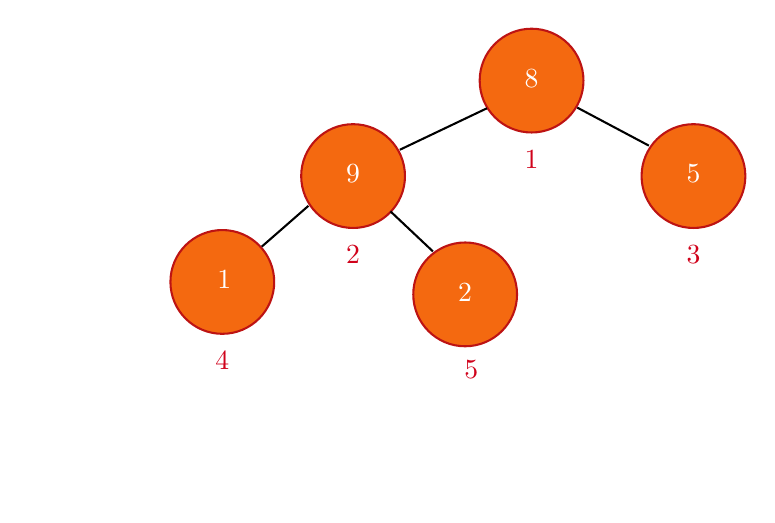
\begin{tikzpicture}[x=0.75pt,y=0.75pt,yscale=-1,xscale=1]
		%uncomment if require: \path (0,300); %set diagram left start at 0, and has height of 300

		\draw  [color={rgb, 255:red, 189; green, 19; blue, 19 }  ,draw opacity=1 ][fill={rgb, 255:red, 244; green, 105; blue, 16 }  ,fill opacity=1 ]  (321, 32) circle [x radius= 25, y radius= 25]  ;
		\draw  [color={rgb, 255:red, 189; green, 19; blue, 19 }  ,draw opacity=1 ][fill={rgb, 255:red, 244; green, 105; blue, 16 }  ,fill opacity=1 ]  (235, 78) circle [x radius= 25, y radius= 25]  ;
		\draw    (257.5,65.33) -- (299.5,45.33) ;


		\draw  [color={rgb, 255:red, 189; green, 19; blue, 19 }  ,draw opacity=1 ][fill={rgb, 255:red, 244; green, 105; blue, 16 }  ,fill opacity=1 ]  (399, 78) circle [x radius= 25, y radius= 25]  ;
		\draw    (343,45) -- (377.5,63.33) ;


		\draw  [color={rgb, 255:red, 189; green, 19; blue, 19 }  ,draw opacity=1 ][fill={rgb, 255:red, 244; green, 105; blue, 16 }  ,fill opacity=1 ]  (172, 129) circle [x radius= 25, y radius= 25]  ;
		\draw    (191,112) -- (213.5,92.33) ;


		\draw  [color={rgb, 255:red, 189; green, 19; blue, 19 }  ,draw opacity=1 ][fill={rgb, 255:red, 244; green, 105; blue, 16 }  ,fill opacity=1 ]  (289, 135) circle [x radius= 25, y radius= 25]  ;
		\draw    (253,95) -- (273.5,114.33) ;



		\draw (321,31) node [color={rgb, 255:red, 255; green, 255; blue, 255 }  ,opacity=1 ] [align=left] {8};
		\draw (321,70) node [color={rgb, 255:red, 208; green, 2; blue, 27 }  ,opacity=1 ] [align=left] {1};
		\draw (235,77) node [color={rgb, 255:red, 255; green, 255; blue, 255 }  ,opacity=1 ] [align=left] {9};
		\draw (235,116) node [color={rgb, 255:red, 208; green, 2; blue, 27 }  ,opacity=1 ] [align=left] {2};
		\draw (399,77) node [color={rgb, 255:red, 255; green, 255; blue, 255 }  ,opacity=1 ] [align=left] {5};
		\draw (399,116) node [color={rgb, 255:red, 208; green, 2; blue, 27 }  ,opacity=1 ] [align=left] {3};
		\draw (173,128) node [color={rgb, 255:red, 255; green, 255; blue, 255 }  ,opacity=1 ] [align=left] {1};
		\draw (172,167) node [color={rgb, 255:red, 208; green, 2; blue, 27 }  ,opacity=1 ] [align=left] {4};
		\draw (86,174) node [color={rgb, 255:red, 255; green, 255; blue, 255 }  ,opacity=1 ] [align=left] {1};
		\draw (250,174) node [color={rgb, 255:red, 255; green, 255; blue, 255 }  ,opacity=1 ] [align=left] {5};
		\draw (289,134) node [color={rgb, 255:red, 255; green, 255; blue, 255 }  ,opacity=1 ] [align=left] {2};
		\draw (292,171) node [color={rgb, 255:red, 208; green, 2; blue, 27 }  ,opacity=1 ] [align=left] {5};
		\draw (304,223) node [color={rgb, 255:red, 255; green, 255; blue, 255 }  ,opacity=1 ] [align=left] {5};

		\end{tikzpicture}
	\end{center}
\end{frame}


\begin{frame}
	\frametitle{Heapify()}
	   \begin{center}
     	\tikzset{every picture/.style={line width=0.75pt}} %set default line width to 0.75pt

     	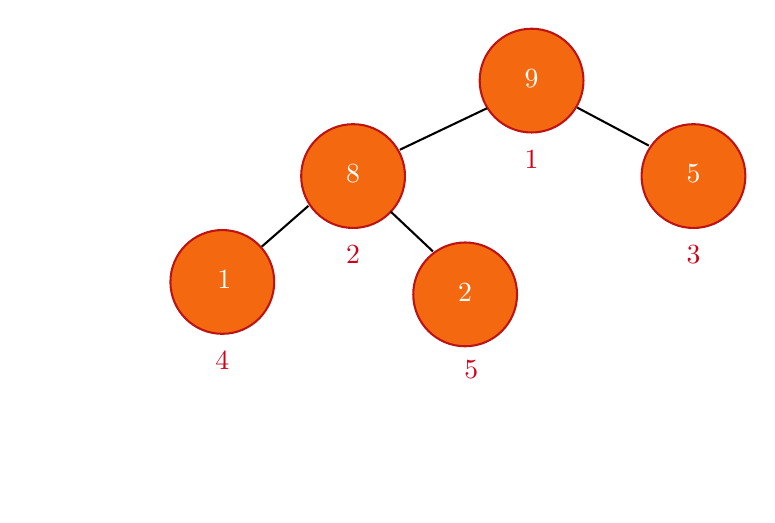
\begin{tikzpicture}[x=0.75pt,y=0.75pt,yscale=-1,xscale=1]
     	%uncomment if require: \path (0,300); %set diagram left start at 0, and has height of 300

     	\draw  [color={rgb, 255:red, 189; green, 19; blue, 19 }  ,draw opacity=1 ][fill={rgb, 255:red, 244; green, 105; blue, 16 }  ,fill opacity=1 ]  (321, 32) circle [x radius= 25, y radius= 25]  ;
     	\draw  [color={rgb, 255:red, 189; green, 19; blue, 19 }  ,draw opacity=1 ][fill={rgb, 255:red, 244; green, 105; blue, 16 }  ,fill opacity=1 ]  (235, 78) circle [x radius= 25, y radius= 25]  ;
     	\draw    (257.5,65.33) -- (299.5,45.33) ;


     	\draw  [color={rgb, 255:red, 189; green, 19; blue, 19 }  ,draw opacity=1 ][fill={rgb, 255:red, 244; green, 105; blue, 16 }  ,fill opacity=1 ]  (399, 78) circle [x radius= 25, y radius= 25]  ;
     	\draw    (343,45) -- (377.5,63.33) ;


     	\draw  [color={rgb, 255:red, 189; green, 19; blue, 19 }  ,draw opacity=1 ][fill={rgb, 255:red, 244; green, 105; blue, 16 }  ,fill opacity=1 ]  (172, 129) circle [x radius= 25, y radius= 25]  ;
     	\draw    (191,112) -- (213.5,92.33) ;


     	\draw  [color={rgb, 255:red, 189; green, 19; blue, 19 }  ,draw opacity=1 ][fill={rgb, 255:red, 244; green, 105; blue, 16 }  ,fill opacity=1 ]  (289, 135) circle [x radius= 25, y radius= 25]  ;
     	\draw    (253,95) -- (273.5,114.33) ;



     	\draw (321,31) node [color={rgb, 255:red, 255; green, 255; blue, 255 }  ,opacity=1 ] [align=left] {9};
     	\draw (321,70) node [color={rgb, 255:red, 208; green, 2; blue, 27 }  ,opacity=1 ] [align=left] {1};
     	\draw (235,77) node [color={rgb, 255:red, 255; green, 255; blue, 255 }  ,opacity=1 ] [align=left] {8};
     	\draw (235,116) node [color={rgb, 255:red, 208; green, 2; blue, 27 }  ,opacity=1 ] [align=left] {2};
     	\draw (399,77) node [color={rgb, 255:red, 255; green, 255; blue, 255 }  ,opacity=1 ] [align=left] {5};
     	\draw (399,116) node [color={rgb, 255:red, 208; green, 2; blue, 27 }  ,opacity=1 ] [align=left] {3};
     	\draw (173,128) node [color={rgb, 255:red, 255; green, 255; blue, 255 }  ,opacity=1 ] [align=left] {1};
     	\draw (172,167) node [color={rgb, 255:red, 208; green, 2; blue, 27 }  ,opacity=1 ] [align=left] {4};
     	\draw (86,174) node [color={rgb, 255:red, 255; green, 255; blue, 255 }  ,opacity=1 ] [align=left] {1};
     	\draw (250,174) node [color={rgb, 255:red, 255; green, 255; blue, 255 }  ,opacity=1 ] [align=left] {5};
     	\draw (289,134) node [color={rgb, 255:red, 255; green, 255; blue, 255 }  ,opacity=1 ] [align=left] {2};
     	\draw (292,171) node [color={rgb, 255:red, 208; green, 2; blue, 27 }  ,opacity=1 ] [align=left] {5};
     	\draw (304,223) node [color={rgb, 255:red, 255; green, 255; blue, 255 }  ,opacity=1 ] [align=left] {5};


     	\end{tikzpicture}
     \end{center}
\end{frame}

\begin{frame}
	\frametitle{Inserting 3}
	\begin{center}
		\tikzset{every picture/.style={line width=0.75pt}} %set default line width to 0.75pt

		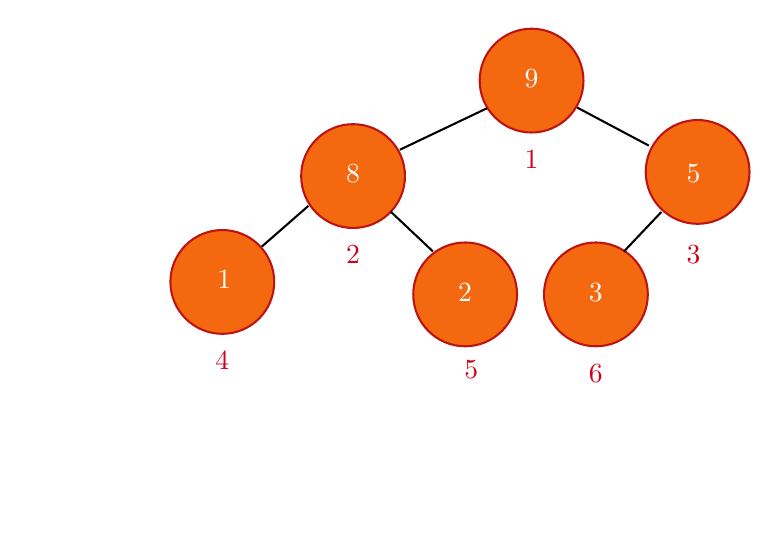
\begin{tikzpicture}[x=0.75pt,y=0.75pt,yscale=-1,xscale=1]
		%uncomment if require: \path (0,300); %set diagram left start at 0, and has height of 300

		\draw  [color={rgb, 255:red, 189; green, 19; blue, 19 }  ,draw opacity=1 ][fill={rgb, 255:red, 244; green, 105; blue, 16 }  ,fill opacity=1 ]  (321, 32) circle [x radius= 25, y radius= 25]  ;
		\draw  [color={rgb, 255:red, 189; green, 19; blue, 19 }  ,draw opacity=1 ][fill={rgb, 255:red, 244; green, 105; blue, 16 }  ,fill opacity=1 ]  (235, 78) circle [x radius= 25, y radius= 25]  ;
		\draw    (257.5,65.33) -- (299.5,45.33) ;


		\draw  [color={rgb, 255:red, 189; green, 19; blue, 19 }  ,draw opacity=1 ][fill={rgb, 255:red, 244; green, 105; blue, 16 }  ,fill opacity=1 ]  (401, 76) circle [x radius= 25, y radius= 25]  ;
		\draw    (343,45) -- (377.5,63.33) ;


		\draw  [color={rgb, 255:red, 189; green, 19; blue, 19 }  ,draw opacity=1 ][fill={rgb, 255:red, 244; green, 105; blue, 16 }  ,fill opacity=1 ]  (172, 129) circle [x radius= 25, y radius= 25]  ;
		\draw    (191,112) -- (213.5,92.33) ;


		\draw  [color={rgb, 255:red, 189; green, 19; blue, 19 }  ,draw opacity=1 ][fill={rgb, 255:red, 244; green, 105; blue, 16 }  ,fill opacity=1 ]  (289, 135) circle [x radius= 25, y radius= 25]  ;
		\draw    (253,95) -- (273.5,114.33) ;


		\draw  [color={rgb, 255:red, 189; green, 19; blue, 19 }  ,draw opacity=1 ][fill={rgb, 255:red, 244; green, 105; blue, 16 }  ,fill opacity=1 ]  (352, 135) circle [x radius= 25, y radius= 25]  ;
		\draw    (365.5,114.33) -- (383.5,95.33) ;



		\draw (321,31) node [color={rgb, 255:red, 255; green, 255; blue, 255 }  ,opacity=1 ] [align=left] {9};
		\draw (321,70) node [color={rgb, 255:red, 208; green, 2; blue, 27 }  ,opacity=1 ] [align=left] {1};
		\draw (235,77) node [color={rgb, 255:red, 255; green, 255; blue, 255 }  ,opacity=1 ] [align=left] {8};
		\draw (235,116) node [color={rgb, 255:red, 208; green, 2; blue, 27 }  ,opacity=1 ] [align=left] {2};
		\draw (399,77) node [color={rgb, 255:red, 255; green, 255; blue, 255 }  ,opacity=1 ] [align=left] {5};
		\draw (399,116) node [color={rgb, 255:red, 208; green, 2; blue, 27 }  ,opacity=1 ] [align=left] {3};
		\draw (173,128) node [color={rgb, 255:red, 255; green, 255; blue, 255 }  ,opacity=1 ] [align=left] {1};
		\draw (172,167) node [color={rgb, 255:red, 208; green, 2; blue, 27 }  ,opacity=1 ] [align=left] {4};
		\draw (86,174) node [color={rgb, 255:red, 255; green, 255; blue, 255 }  ,opacity=1 ] [align=left] {1};
		\draw (250,174) node [color={rgb, 255:red, 255; green, 255; blue, 255 }  ,opacity=1 ] [align=left] {5};
		\draw (289,134) node [color={rgb, 255:red, 255; green, 255; blue, 255 }  ,opacity=1 ] [align=left] {2};
		\draw (292,171) node [color={rgb, 255:red, 208; green, 2; blue, 27 }  ,opacity=1 ] [align=left] {5};
		\draw (352,134) node [color={rgb, 255:red, 255; green, 255; blue, 255 }  ,opacity=1 ] [align=left] {3};
		\draw (352,173) node [color={rgb, 255:red, 208; green, 2; blue, 27 }  ,opacity=1 ] [align=left] {6};
		\draw (290,185) node [color={rgb, 255:red, 255; green, 255; blue, 255 }  ,opacity=1 ] [align=left] {1};
		\draw (367,231) node [color={rgb, 255:red, 255; green, 255; blue, 255 }  ,opacity=1 ] [align=left] {5};


		\end{tikzpicture}
	\end{center}
\end{frame}


\begin{frame}
	\frametitle{Inserting 12}

	\begin{center}
		\tikzset{every picture/.style={line width=0.75pt}} %set default line width to 0.75pt

		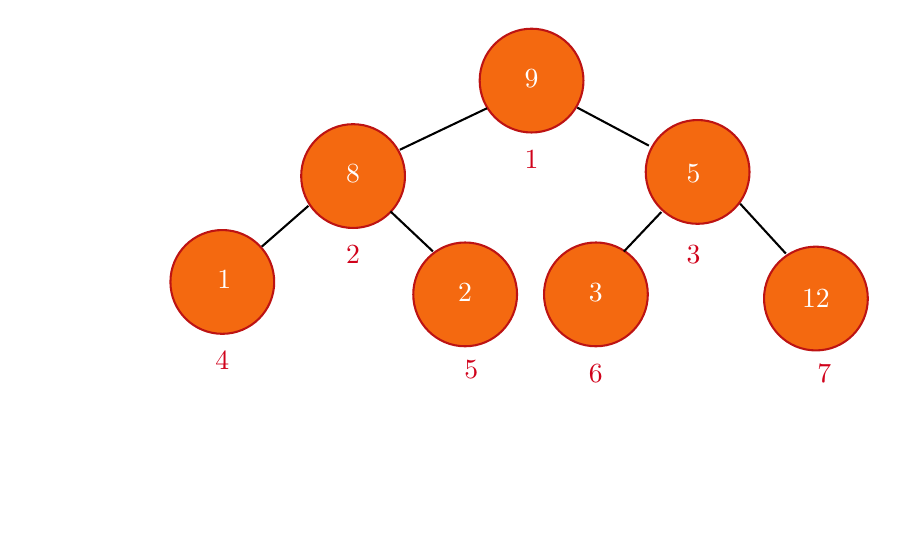
\begin{tikzpicture}[x=0.75pt,y=0.75pt,yscale=-1,xscale=1]
		%uncomment if require: \path (0,300); %set diagram left start at 0, and has height of 300

		\draw  [color={rgb, 255:red, 189; green, 19; blue, 19 }  ,draw opacity=1 ][fill={rgb, 255:red, 244; green, 105; blue, 16 }  ,fill opacity=1 ]  (321, 32) circle [x radius= 25, y radius= 25]  ;
		\draw  [color={rgb, 255:red, 189; green, 19; blue, 19 }  ,draw opacity=1 ][fill={rgb, 255:red, 244; green, 105; blue, 16 }  ,fill opacity=1 ]  (235, 78) circle [x radius= 25, y radius= 25]  ;
		\draw    (257.5,65.33) -- (299.5,45.33) ;


		\draw  [color={rgb, 255:red, 189; green, 19; blue, 19 }  ,draw opacity=1 ][fill={rgb, 255:red, 244; green, 105; blue, 16 }  ,fill opacity=1 ]  (401, 76) circle [x radius= 25, y radius= 25]  ;
		\draw    (343,45) -- (377.5,63.33) ;


		\draw  [color={rgb, 255:red, 189; green, 19; blue, 19 }  ,draw opacity=1 ][fill={rgb, 255:red, 244; green, 105; blue, 16 }  ,fill opacity=1 ]  (172, 129) circle [x radius= 25, y radius= 25]  ;
		\draw    (191,112) -- (213.5,92.33) ;


		\draw  [color={rgb, 255:red, 189; green, 19; blue, 19 }  ,draw opacity=1 ][fill={rgb, 255:red, 244; green, 105; blue, 16 }  ,fill opacity=1 ]  (289, 135) circle [x radius= 25, y radius= 25]  ;
		\draw    (253,95) -- (273.5,114.33) ;


		\draw  [color={rgb, 255:red, 189; green, 19; blue, 19 }  ,draw opacity=1 ][fill={rgb, 255:red, 244; green, 105; blue, 16 }  ,fill opacity=1 ]  (352, 135) circle [x radius= 25, y radius= 25]  ;
		\draw    (365.5,114.33) -- (383.5,95.33) ;


		\draw  [color={rgb, 255:red, 189; green, 19; blue, 19 }  ,draw opacity=1 ][fill={rgb, 255:red, 244; green, 105; blue, 16 }  ,fill opacity=1 ]  (458, 137) circle [x radius= 25, y radius= 25]  ;
		\draw    (421.5,91.33) -- (443.5,115.33) ;



		\draw (321,31) node [color={rgb, 255:red, 255; green, 255; blue, 255 }  ,opacity=1 ] [align=left] {9};
		\draw (321,70) node [color={rgb, 255:red, 208; green, 2; blue, 27 }  ,opacity=1 ] [align=left] {1};
		\draw (235,77) node [color={rgb, 255:red, 255; green, 255; blue, 255 }  ,opacity=1 ] [align=left] {8};
		\draw (235,116) node [color={rgb, 255:red, 208; green, 2; blue, 27 }  ,opacity=1 ] [align=left] {2};
		\draw (399,77) node [color={rgb, 255:red, 255; green, 255; blue, 255 }  ,opacity=1 ] [align=left] {5};
		\draw (399,116) node [color={rgb, 255:red, 208; green, 2; blue, 27 }  ,opacity=1 ] [align=left] {3};
		\draw (173,128) node [color={rgb, 255:red, 255; green, 255; blue, 255 }  ,opacity=1 ] [align=left] {1};
		\draw (172,167) node [color={rgb, 255:red, 208; green, 2; blue, 27 }  ,opacity=1 ] [align=left] {4};
		\draw (86,174) node [color={rgb, 255:red, 255; green, 255; blue, 255 }  ,opacity=1 ] [align=left] {1};
		\draw (250,174) node [color={rgb, 255:red, 255; green, 255; blue, 255 }  ,opacity=1 ] [align=left] {5};
		\draw (289,134) node [color={rgb, 255:red, 255; green, 255; blue, 255 }  ,opacity=1 ] [align=left] {2};
		\draw (292,171) node [color={rgb, 255:red, 208; green, 2; blue, 27 }  ,opacity=1 ] [align=left] {5};
		\draw (352,134) node [color={rgb, 255:red, 255; green, 255; blue, 255 }  ,opacity=1 ] [align=left] {3};
		\draw (352,173) node [color={rgb, 255:red, 208; green, 2; blue, 27 }  ,opacity=1 ] [align=left] {6};
		\draw (290,185) node [color={rgb, 255:red, 255; green, 255; blue, 255 }  ,opacity=1 ] [align=left] {1};
		\draw (367,231) node [color={rgb, 255:red, 255; green, 255; blue, 255 }  ,opacity=1 ] [align=left] {5};
		\draw (458,137) node [color={rgb, 255:red, 255; green, 255; blue, 255 }  ,opacity=1 ] [align=left] {12};
		\draw (462,173) node [color={rgb, 255:red, 208; green, 2; blue, 27 }  ,opacity=1 ] [align=left] {7};


		\end{tikzpicture}
	\end{center}
\end{frame}

\begin{frame}
	\frametitle{Heapify()}
	  \begin{center}
    	\tikzset{every picture/.style={line width=0.75pt}} %set default line width to 0.75pt

    	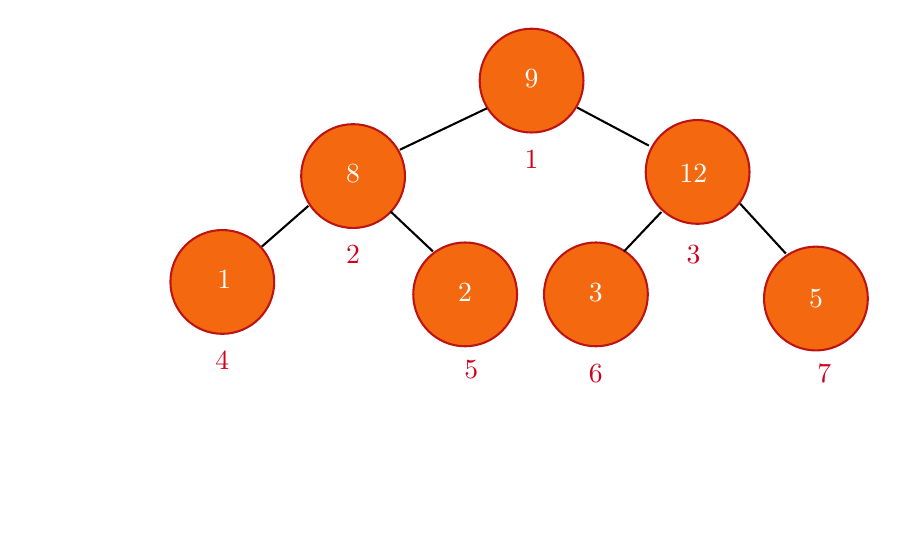
\begin{tikzpicture}[x=0.75pt,y=0.75pt,yscale=-1,xscale=1]
    	%uncomment if require: \path (0,300); %set diagram left start at 0, and has height of 300

    	\draw  [color={rgb, 255:red, 189; green, 19; blue, 19 }  ,draw opacity=1 ][fill={rgb, 255:red, 244; green, 105; blue, 16 }  ,fill opacity=1 ]  (321, 32) circle [x radius= 25, y radius= 25]  ;
    	\draw  [color={rgb, 255:red, 189; green, 19; blue, 19 }  ,draw opacity=1 ][fill={rgb, 255:red, 244; green, 105; blue, 16 }  ,fill opacity=1 ]  (235, 78) circle [x radius= 25, y radius= 25]  ;
    	\draw    (257.5,65.33) -- (299.5,45.33) ;


    	\draw  [color={rgb, 255:red, 189; green, 19; blue, 19 }  ,draw opacity=1 ][fill={rgb, 255:red, 244; green, 105; blue, 16 }  ,fill opacity=1 ]  (401, 76) circle [x radius= 25, y radius= 25]  ;
    	\draw    (343,45) -- (377.5,63.33) ;


    	\draw  [color={rgb, 255:red, 189; green, 19; blue, 19 }  ,draw opacity=1 ][fill={rgb, 255:red, 244; green, 105; blue, 16 }  ,fill opacity=1 ]  (172, 129) circle [x radius= 25, y radius= 25]  ;
    	\draw    (191,112) -- (213.5,92.33) ;


    	\draw  [color={rgb, 255:red, 189; green, 19; blue, 19 }  ,draw opacity=1 ][fill={rgb, 255:red, 244; green, 105; blue, 16 }  ,fill opacity=1 ]  (289, 135) circle [x radius= 25, y radius= 25]  ;
    	\draw    (253,95) -- (273.5,114.33) ;


    	\draw  [color={rgb, 255:red, 189; green, 19; blue, 19 }  ,draw opacity=1 ][fill={rgb, 255:red, 244; green, 105; blue, 16 }  ,fill opacity=1 ]  (352, 135) circle [x radius= 25, y radius= 25]  ;
    	\draw    (365.5,114.33) -- (383.5,95.33) ;


    	\draw  [color={rgb, 255:red, 189; green, 19; blue, 19 }  ,draw opacity=1 ][fill={rgb, 255:red, 244; green, 105; blue, 16 }  ,fill opacity=1 ]  (458, 137) circle [x radius= 25, y radius= 25]  ;
    	\draw    (421.5,91.33) -- (443.5,115.33) ;



    	\draw (321,31) node [color={rgb, 255:red, 255; green, 255; blue, 255 }  ,opacity=1 ] [align=left] {9};
    	\draw (321,70) node [color={rgb, 255:red, 208; green, 2; blue, 27 }  ,opacity=1 ] [align=left] {1};
    	\draw (235,77) node [color={rgb, 255:red, 255; green, 255; blue, 255 }  ,opacity=1 ] [align=left] {8};
    	\draw (235,116) node [color={rgb, 255:red, 208; green, 2; blue, 27 }  ,opacity=1 ] [align=left] {2};
    	\draw (399,77) node [color={rgb, 255:red, 255; green, 255; blue, 255 }  ,opacity=1 ] [align=left] {12};
    	\draw (399,116) node [color={rgb, 255:red, 208; green, 2; blue, 27 }  ,opacity=1 ] [align=left] {3};
    	\draw (173,128) node [color={rgb, 255:red, 255; green, 255; blue, 255 }  ,opacity=1 ] [align=left] {1};
    	\draw (172,167) node [color={rgb, 255:red, 208; green, 2; blue, 27 }  ,opacity=1 ] [align=left] {4};
    	\draw (86,174) node [color={rgb, 255:red, 255; green, 255; blue, 255 }  ,opacity=1 ] [align=left] {1};
    	\draw (250,174) node [color={rgb, 255:red, 255; green, 255; blue, 255 }  ,opacity=1 ] [align=left] {5};
    	\draw (289,134) node [color={rgb, 255:red, 255; green, 255; blue, 255 }  ,opacity=1 ] [align=left] {2};
    	\draw (292,171) node [color={rgb, 255:red, 208; green, 2; blue, 27 }  ,opacity=1 ] [align=left] {5};
    	\draw (352,134) node [color={rgb, 255:red, 255; green, 255; blue, 255 }  ,opacity=1 ] [align=left] {3};
    	\draw (352,173) node [color={rgb, 255:red, 208; green, 2; blue, 27 }  ,opacity=1 ] [align=left] {6};
    	\draw (290,185) node [color={rgb, 255:red, 255; green, 255; blue, 255 }  ,opacity=1 ] [align=left] {1};
    	\draw (367,231) node [color={rgb, 255:red, 255; green, 255; blue, 255 }  ,opacity=1 ] [align=left] {5};
    	\draw (458,137) node [color={rgb, 255:red, 255; green, 255; blue, 255 }  ,opacity=1 ] [align=left] {5};
    	\draw (462,173) node [color={rgb, 255:red, 208; green, 2; blue, 27 }  ,opacity=1 ] [align=left] {7};


    	\end{tikzpicture}
    \end{center}
\end{frame}


\begin{frame}
	\frametitle{Heapify()}
	\begin{center}
		\tikzset{every picture/.style={line width=0.75pt}} %set default line width to 0.75pt

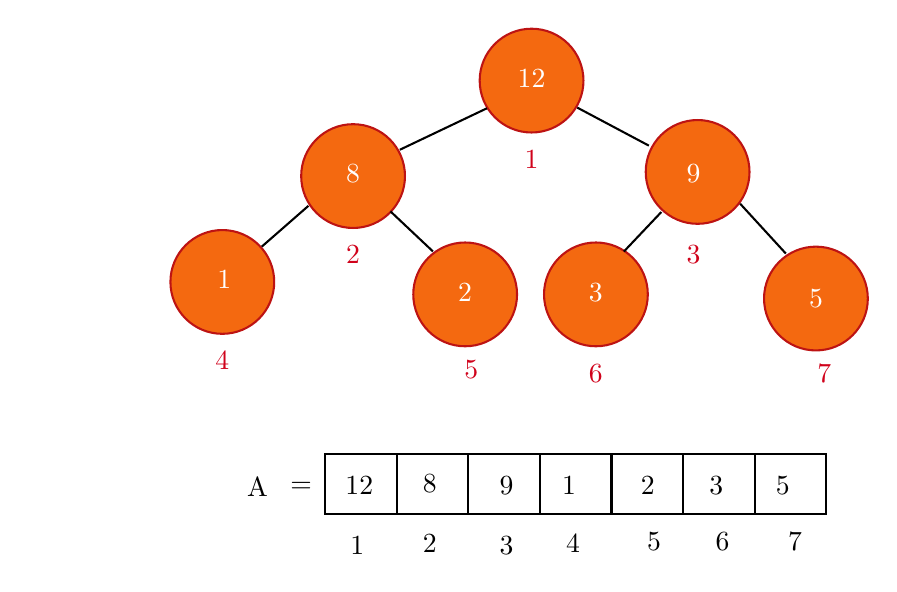
\begin{tikzpicture}[x=0.75pt,y=0.75pt,yscale=-1,xscale=1]
%uncomment if require: \path (0,300); %set diagram left start at 0, and has height of 300

\draw  [color={rgb, 255:red, 189; green, 19; blue, 19 }  ,draw opacity=1 ][fill={rgb, 255:red, 244; green, 105; blue, 16 }  ,fill opacity=1 ]  (321, 32) circle [x radius= 25, y radius= 25]  ;
\draw  [color={rgb, 255:red, 189; green, 19; blue, 19 }  ,draw opacity=1 ][fill={rgb, 255:red, 244; green, 105; blue, 16 }  ,fill opacity=1 ]  (235, 78) circle [x radius= 25, y radius= 25]  ;
\draw    (257.5,65.33) -- (299.5,45.33) ;


\draw  [color={rgb, 255:red, 189; green, 19; blue, 19 }  ,draw opacity=1 ][fill={rgb, 255:red, 244; green, 105; blue, 16 }  ,fill opacity=1 ]  (401, 76) circle [x radius= 25, y radius= 25]  ;
\draw    (343,45) -- (377.5,63.33) ;


\draw  [color={rgb, 255:red, 189; green, 19; blue, 19 }  ,draw opacity=1 ][fill={rgb, 255:red, 244; green, 105; blue, 16 }  ,fill opacity=1 ]  (172, 129) circle [x radius= 25, y radius= 25]  ;
\draw    (191,112) -- (213.5,92.33) ;


\draw  [color={rgb, 255:red, 189; green, 19; blue, 19 }  ,draw opacity=1 ][fill={rgb, 255:red, 244; green, 105; blue, 16 }  ,fill opacity=1 ]  (289, 135) circle [x radius= 25, y radius= 25]  ;
\draw    (253,95) -- (273.5,114.33) ;


\draw  [color={rgb, 255:red, 189; green, 19; blue, 19 }  ,draw opacity=1 ][fill={rgb, 255:red, 244; green, 105; blue, 16 }  ,fill opacity=1 ]  (352, 135) circle [x radius= 25, y radius= 25]  ;
\draw    (365.5,114.33) -- (383.5,95.33) ;


\draw  [color={rgb, 255:red, 189; green, 19; blue, 19 }  ,draw opacity=1 ][fill={rgb, 255:red, 244; green, 105; blue, 16 }  ,fill opacity=1 ]  (458, 137) circle [x radius= 25, y radius= 25]  ;
\draw    (421.5,91.33) -- (443.5,115.33) ;


\draw    (290.5, 212) rectangle (325, 240.67)   ;
\draw    (394, 212) rectangle (428.5, 240.67)   ;
\draw    (359.5, 212) rectangle (394, 240.67)   ;
\draw    (221.5, 212) rectangle (256, 240.67)   ;
\draw    (256, 212) rectangle (290.5, 240.67)   ;
\draw    (428.5, 212) rectangle (463, 240.67)   ;
\draw    (325, 212) rectangle (359.5, 240.67)   ;

\draw (321,31) node [color={rgb, 255:red, 255; green, 255; blue, 255 }  ,opacity=1 ] [align=left] {12};
\draw (321,70) node [color={rgb, 255:red, 208; green, 2; blue, 27 }  ,opacity=1 ] [align=left] {1};
\draw (235,77) node [color={rgb, 255:red, 255; green, 255; blue, 255 }  ,opacity=1 ] [align=left] {8};
\draw (235,116) node [color={rgb, 255:red, 208; green, 2; blue, 27 }  ,opacity=1 ] [align=left] {2};
\draw (399,77) node [color={rgb, 255:red, 255; green, 255; blue, 255 }  ,opacity=1 ] [align=left] {9};
\draw (399,116) node [color={rgb, 255:red, 208; green, 2; blue, 27 }  ,opacity=1 ] [align=left] {3};
\draw (173,128) node [color={rgb, 255:red, 255; green, 255; blue, 255 }  ,opacity=1 ] [align=left] {1};
\draw (172,167) node [color={rgb, 255:red, 208; green, 2; blue, 27 }  ,opacity=1 ] [align=left] {4};
\draw (86,174) node [color={rgb, 255:red, 255; green, 255; blue, 255 }  ,opacity=1 ] [align=left] {1};
\draw (250,174) node [color={rgb, 255:red, 255; green, 255; blue, 255 }  ,opacity=1 ] [align=left] {5};
\draw (289,134) node [color={rgb, 255:red, 255; green, 255; blue, 255 }  ,opacity=1 ] [align=left] {2};
\draw (292,171) node [color={rgb, 255:red, 208; green, 2; blue, 27 }  ,opacity=1 ] [align=left] {5};
\draw (352,134) node [color={rgb, 255:red, 255; green, 255; blue, 255 }  ,opacity=1 ] [align=left] {3};
\draw (352,173) node [color={rgb, 255:red, 208; green, 2; blue, 27 }  ,opacity=1 ] [align=left] {6};
\draw (290,185) node [color={rgb, 255:red, 255; green, 255; blue, 255 }  ,opacity=1 ] [align=left] {1};
\draw (367,231) node [color={rgb, 255:red, 255; green, 255; blue, 255 }  ,opacity=1 ] [align=left] {5};
\draw (458,137) node [color={rgb, 255:red, 255; green, 255; blue, 255 }  ,opacity=1 ] [align=left] {5};
\draw (462,173) node [color={rgb, 255:red, 208; green, 2; blue, 27 }  ,opacity=1 ] [align=left] {7};
\draw (189,228) node  [align=left] {A};
\draw (210,228) node  [align=left] {=};
\draw (238,227) node  [align=left] {12};
\draw (272,226) node  [align=left] {8};
\draw (309,227) node  [align=left] {9};
\draw (339,227) node  [align=left] {1};
\draw (377,227) node  [align=left] {2};
\draw (410,227) node  [align=left] {3};
\draw (442,227) node  [align=left] {5};
\draw (237,256) node  [align=left] {1};
\draw (272,255) node  [align=left] {2};
\draw (309,256) node  [align=left] {3};
\draw (448,254) node  [align=left] {7};
\draw (413,254) node  [align=left] {6};
\draw (380,254) node  [align=left] {5};
\draw (341,255) node  [align=left] {4};


\end{tikzpicture}
	\end{center}


\end{frame}

\begin{frame}
	\frametitle{Extract Max}
	\begin{center}
		\tikzset{every picture/.style={line width=0.75pt}} %set default line width to 0.75pt

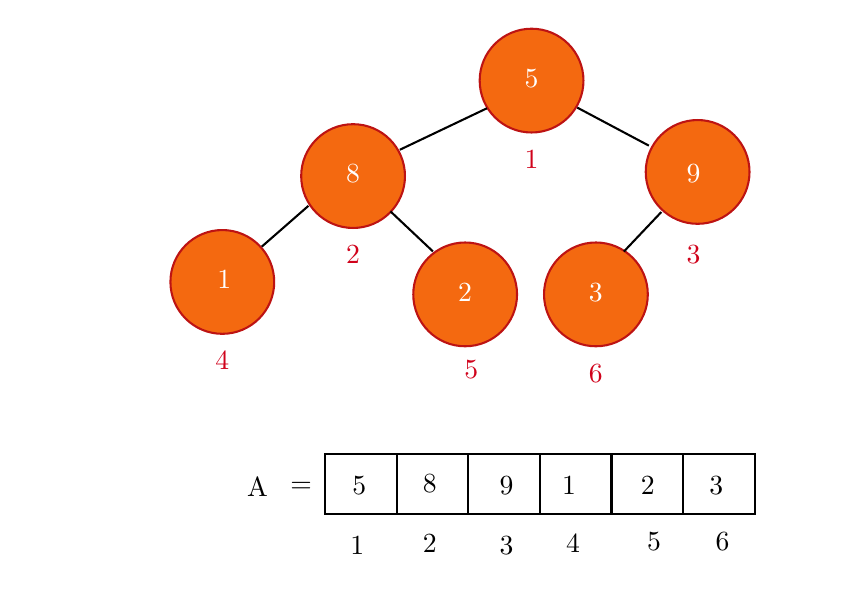
\begin{tikzpicture}[x=0.75pt,y=0.75pt,yscale=-1,xscale=1]
%uncomment if require: \path (0,300); %set diagram left start at 0, and has height of 300

\draw  [color={rgb, 255:red, 189; green, 19; blue, 19 }  ,draw opacity=1 ][fill={rgb, 255:red, 244; green, 105; blue, 16 }  ,fill opacity=1 ]  (321, 32) circle [x radius= 25, y radius= 25]  ;
\draw  [color={rgb, 255:red, 189; green, 19; blue, 19 }  ,draw opacity=1 ][fill={rgb, 255:red, 244; green, 105; blue, 16 }  ,fill opacity=1 ]  (235, 78) circle [x radius= 25, y radius= 25]  ;
\draw    (257.5,65.33) -- (299.5,45.33) ;


\draw  [color={rgb, 255:red, 189; green, 19; blue, 19 }  ,draw opacity=1 ][fill={rgb, 255:red, 244; green, 105; blue, 16 }  ,fill opacity=1 ]  (401, 76) circle [x radius= 25, y radius= 25]  ;
\draw    (343,45) -- (377.5,63.33) ;


\draw  [color={rgb, 255:red, 189; green, 19; blue, 19 }  ,draw opacity=1 ][fill={rgb, 255:red, 244; green, 105; blue, 16 }  ,fill opacity=1 ]  (172, 129) circle [x radius= 25, y radius= 25]  ;
\draw    (191,112) -- (213.5,92.33) ;


\draw  [color={rgb, 255:red, 189; green, 19; blue, 19 }  ,draw opacity=1 ][fill={rgb, 255:red, 244; green, 105; blue, 16 }  ,fill opacity=1 ]  (289, 135) circle [x radius= 25, y radius= 25]  ;
\draw    (253,95) -- (273.5,114.33) ;


\draw  [color={rgb, 255:red, 189; green, 19; blue, 19 }  ,draw opacity=1 ][fill={rgb, 255:red, 244; green, 105; blue, 16 }  ,fill opacity=1 ]  (352, 135) circle [x radius= 25, y radius= 25]  ;
\draw    (365.5,114.33) -- (383.5,95.33) ;


\draw    (290.5, 212) rectangle (325, 240.67)   ;
\draw    (394, 212) rectangle (428.5, 240.67)   ;
\draw    (359.5, 212) rectangle (394, 240.67)   ;
\draw    (221.5, 212) rectangle (256, 240.67)   ;
\draw    (256, 212) rectangle (290.5, 240.67)   ;
\draw    (325, 212) rectangle (359.5, 240.67)   ;

\draw (321,31) node [color={rgb, 255:red, 255; green, 255; blue, 255 }  ,opacity=1 ] [align=left] {5};
\draw (321,70) node [color={rgb, 255:red, 208; green, 2; blue, 27 }  ,opacity=1 ] [align=left] {1};
\draw (235,77) node [color={rgb, 255:red, 255; green, 255; blue, 255 }  ,opacity=1 ] [align=left] {8};
\draw (235,116) node [color={rgb, 255:red, 208; green, 2; blue, 27 }  ,opacity=1 ] [align=left] {2};
\draw (399,77) node [color={rgb, 255:red, 255; green, 255; blue, 255 }  ,opacity=1 ] [align=left] {9};
\draw (399,116) node [color={rgb, 255:red, 208; green, 2; blue, 27 }  ,opacity=1 ] [align=left] {3};
\draw (173,128) node [color={rgb, 255:red, 255; green, 255; blue, 255 }  ,opacity=1 ] [align=left] {1};
\draw (172,167) node [color={rgb, 255:red, 208; green, 2; blue, 27 }  ,opacity=1 ] [align=left] {4};
\draw (86,174) node [color={rgb, 255:red, 255; green, 255; blue, 255 }  ,opacity=1 ] [align=left] {1};
\draw (250,174) node [color={rgb, 255:red, 255; green, 255; blue, 255 }  ,opacity=1 ] [align=left] {5};
\draw (289,134) node [color={rgb, 255:red, 255; green, 255; blue, 255 }  ,opacity=1 ] [align=left] {2};
\draw (292,171) node [color={rgb, 255:red, 208; green, 2; blue, 27 }  ,opacity=1 ] [align=left] {5};
\draw (352,134) node [color={rgb, 255:red, 255; green, 255; blue, 255 }  ,opacity=1 ] [align=left] {3};
\draw (352,173) node [color={rgb, 255:red, 208; green, 2; blue, 27 }  ,opacity=1 ] [align=left] {6};
\draw (290,185) node [color={rgb, 255:red, 255; green, 255; blue, 255 }  ,opacity=1 ] [align=left] {1};
\draw (367,231) node [color={rgb, 255:red, 255; green, 255; blue, 255 }  ,opacity=1 ] [align=left] {5};
\draw (458,137) node [color={rgb, 255:red, 255; green, 255; blue, 255 }  ,opacity=1 ] [align=left] {5};
\draw (189,228) node  [align=left] {A};
\draw (210,228) node  [align=left] {=};
\draw (238,227) node  [align=left] {5};
\draw (272,226) node  [align=left] {8};
\draw (309,227) node  [align=left] {9};
\draw (339,227) node  [align=left] {1};
\draw (377,227) node  [align=left] {2};
\draw (410,227) node  [align=left] {3};
\draw (237,256) node  [align=left] {1};
\draw (272,255) node  [align=left] {2};
\draw (309,256) node  [align=left] {3};
\draw (413,254) node  [align=left] {6};
\draw (380,254) node  [align=left] {5};
\draw (341,255) node  [align=left] {4};


\end{tikzpicture}
	\end{center}

\end{frame}

\begin{frame}
\frametitle{Heapify()}
\begin{center}
	\tikzset{every picture/.style={line width=0.75pt}} %set default line width to 0.75pt

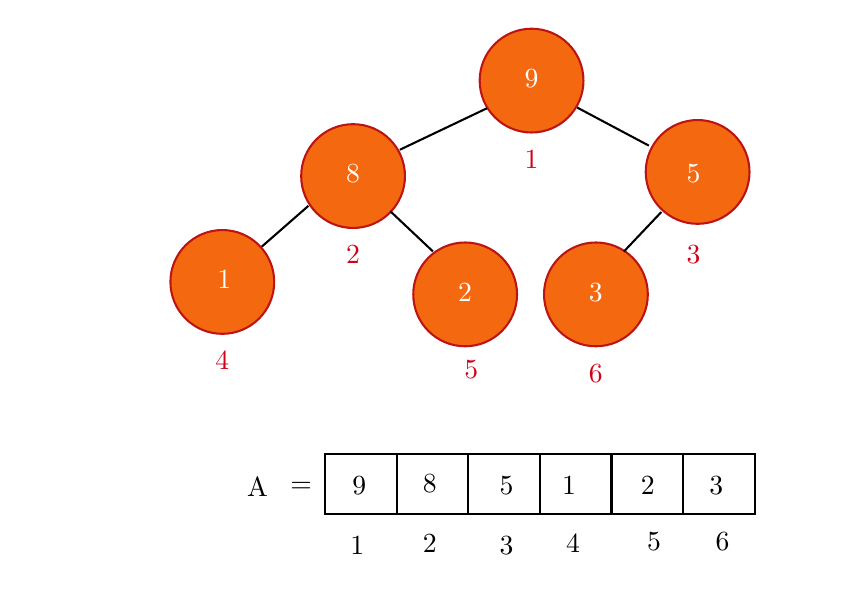
\begin{tikzpicture}[x=0.75pt,y=0.75pt,yscale=-1,xscale=1]
%uncomment if require: \path (0,300); %set diagram left start at 0, and has height of 300

\draw  [color={rgb, 255:red, 189; green, 19; blue, 19 }  ,draw opacity=1 ][fill={rgb, 255:red, 244; green, 105; blue, 16 }  ,fill opacity=1 ]  (321, 32) circle [x radius= 25, y radius= 25]  ;
\draw  [color={rgb, 255:red, 189; green, 19; blue, 19 }  ,draw opacity=1 ][fill={rgb, 255:red, 244; green, 105; blue, 16 }  ,fill opacity=1 ]  (235, 78) circle [x radius= 25, y radius= 25]  ;
\draw    (257.5,65.33) -- (299.5,45.33) ;


\draw  [color={rgb, 255:red, 189; green, 19; blue, 19 }  ,draw opacity=1 ][fill={rgb, 255:red, 244; green, 105; blue, 16 }  ,fill opacity=1 ]  (401, 76) circle [x radius= 25, y radius= 25]  ;
\draw    (343,45) -- (377.5,63.33) ;


\draw  [color={rgb, 255:red, 189; green, 19; blue, 19 }  ,draw opacity=1 ][fill={rgb, 255:red, 244; green, 105; blue, 16 }  ,fill opacity=1 ]  (172, 129) circle [x radius= 25, y radius= 25]  ;
\draw    (191,112) -- (213.5,92.33) ;


\draw  [color={rgb, 255:red, 189; green, 19; blue, 19 }  ,draw opacity=1 ][fill={rgb, 255:red, 244; green, 105; blue, 16 }  ,fill opacity=1 ]  (289, 135) circle [x radius= 25, y radius= 25]  ;
\draw    (253,95) -- (273.5,114.33) ;


\draw  [color={rgb, 255:red, 189; green, 19; blue, 19 }  ,draw opacity=1 ][fill={rgb, 255:red, 244; green, 105; blue, 16 }  ,fill opacity=1 ]  (352, 135) circle [x radius= 25, y radius= 25]  ;
\draw    (365.5,114.33) -- (383.5,95.33) ;


\draw    (290.5, 212) rectangle (325, 240.67)   ;
\draw    (394, 212) rectangle (428.5, 240.67)   ;
\draw    (359.5, 212) rectangle (394, 240.67)   ;
\draw    (221.5, 212) rectangle (256, 240.67)   ;
\draw    (256, 212) rectangle (290.5, 240.67)   ;
\draw    (325, 212) rectangle (359.5, 240.67)   ;

\draw (321,31) node [color={rgb, 255:red, 255; green, 255; blue, 255 }  ,opacity=1 ] [align=left] {9};
\draw (321,70) node [color={rgb, 255:red, 208; green, 2; blue, 27 }  ,opacity=1 ] [align=left] {1};
\draw (235,77) node [color={rgb, 255:red, 255; green, 255; blue, 255 }  ,opacity=1 ] [align=left] {8};
\draw (235,116) node [color={rgb, 255:red, 208; green, 2; blue, 27 }  ,opacity=1 ] [align=left] {2};
\draw (399,77) node [color={rgb, 255:red, 255; green, 255; blue, 255 }  ,opacity=1 ] [align=left] {5};
\draw (399,116) node [color={rgb, 255:red, 208; green, 2; blue, 27 }  ,opacity=1 ] [align=left] {3};
\draw (173,128) node [color={rgb, 255:red, 255; green, 255; blue, 255 }  ,opacity=1 ] [align=left] {1};
\draw (172,167) node [color={rgb, 255:red, 208; green, 2; blue, 27 }  ,opacity=1 ] [align=left] {4};
\draw (86,174) node [color={rgb, 255:red, 255; green, 255; blue, 255 }  ,opacity=1 ] [align=left] {1};
\draw (250,174) node [color={rgb, 255:red, 255; green, 255; blue, 255 }  ,opacity=1 ] [align=left] {5};
\draw (289,134) node [color={rgb, 255:red, 255; green, 255; blue, 255 }  ,opacity=1 ] [align=left] {2};
\draw (292,171) node [color={rgb, 255:red, 208; green, 2; blue, 27 }  ,opacity=1 ] [align=left] {5};
\draw (352,134) node [color={rgb, 255:red, 255; green, 255; blue, 255 }  ,opacity=1 ] [align=left] {3};
\draw (352,173) node [color={rgb, 255:red, 208; green, 2; blue, 27 }  ,opacity=1 ] [align=left] {6};
\draw (290,185) node [color={rgb, 255:red, 255; green, 255; blue, 255 }  ,opacity=1 ] [align=left] {1};
\draw (367,231) node [color={rgb, 255:red, 255; green, 255; blue, 255 }  ,opacity=1 ] [align=left] {5};
\draw (458,137) node [color={rgb, 255:red, 255; green, 255; blue, 255 }  ,opacity=1 ] [align=left] {5};
\draw (189,228) node  [align=left] {A};
\draw (210,228) node  [align=left] {=};
\draw (238,227) node  [align=left] {9};
\draw (272,226) node  [align=left] {8};
\draw (309,227) node  [align=left] {5};
\draw (339,227) node  [align=left] {1};
\draw (377,227) node  [align=left] {2};
\draw (410,227) node  [align=left] {3};
\draw (237,256) node  [align=left] {1};
\draw (272,255) node  [align=left] {2};
\draw (309,256) node  [align=left] {3};
\draw (413,254) node  [align=left] {6};
\draw (380,254) node  [align=left] {5};
\draw (341,255) node  [align=left] {4};


\end{tikzpicture}
\end{center}
\end{frame}
